% ============================================================
%  chapters/ch03a.tex —— 第三章 超流性（前半）：§22–§28
%  印刷页 78–105（PDF 物理页 p089–p112）
%  插图：图 2（PDF p091，液氦元激发色散律；占位 figures/fig2.pdf）
%  圈码脚注标记：21 处/19 行已全部转录为 \footnote{...}（§22:2、§23:6、
%    习题:1、§24:2、§25:2、§26:5、§27:1、§28:1——分别位于 p089×2、p090、
%    p091、p093、p095×3、p097、p098、p099、p101×2、p104、p105×2、p106×2、
%    p107、p108、p110），脚注文本按 原书转换/pages 相应页面 300dpi 渲染逐字
%    转录；原书脚注按页重编号（每页自①起），与 \footnote 按页自动复位一致；
%    任务书"圈码 17 行"指 OCR 字面行数，OCR 有 2 处圈码变形：
%    \textcircled{1}（p095 ①）与 \mathcal{Q}（p101 ②），已照页面还原
%  已修正的 OCR/原书错误（编号：依据页面 pNNN）：
%   1. p089 首锚点 %%p 088 系切片错位，§22 实起于 PDF p089（印刷页78）；
%      自 %%p 090 起锚点与 PDF 页一致
%   2. p090 (22.2) OCR \v{p} 还原为 \bm p；(22.3) 分母 \mu 还原为 u，
%      即 90(\hbar u)^3（页面明确印作 (hu)）
%   3. p090 "大干原子间距" → "大于"（照页面）
%   4. p091 (22.7) 原书排印 "m^* = 0.14 米(^4He)"（"米"显系 m 之误排），
%      照原书排入，未改动
%   5. p091–92 (22.8)(22.9)(22.10) 及正文 F_旋、S_旋、C_旋 的中文下标
%      "旋"，OCR 乱码（𝔛、fif、\hbar\hat\varepsilon 等）照页面还原
%   6. p092–93 §23 速度 v OCR 误作 σ/υ多处，均还原为 \bm v（含 23.1 前后文）
%   7. p092 "在这个坐标系中氮是静止的" → "氦"（照页面）
%   8. p094 "我们得知：就存在一部分……" → "只存在"（照页面）
%   9. p095–96 §23 末文献 OCR "..∏y，.., 1948]" 还原为
%      [Л. Д. Ландау, И. Я. Померанчук, 1948]（跨页 p095–96）
%  10. p095 (23.6)(23.7)(23.8) OCR \rho_{\ast}→\rho_n；E_{ps}→E_声；
%      (ρ_n)_声/(ρ_n)_旋 中文下标照页面还原
%  11. p096 (23.9)(23.10) ε_杂、m*_杂、N_杂 照页面还原；"2,8" → "2.8"
%  12. p096 习题1 解 OCR 漏句"（式中积分具有迅速的收敛性，因此允许将
%      积分上限换成无穷大）. 算出积分"，照 p096 页面补入
%  13. p097 习题2 色散律记号 \varepsilon_{\hbar*} → ε_杂（照页面）
%  14. p099 §24 速度算符 OCR 误作 θ/ϑ 多处 → \hat{\bm v}（照页面）
%  15. p099–100 (24.10) 前一式 OCR "e^{i(t·r−ukt)}"、占位符 λ →
%      e^{i(\bm k·\bm r−kut)}（照 p099–100 页面）
%  16. p101 (24.12)(24.13) 导数算符 \pmb{\rho}_0 → \rho_0（下标 0 正体，
%      照页面）
%  17. p101 (25.1) 首项 OCR 漏产生算符上标 → \hat a^+_{\bm p}\hat a_{\bm p}
%      （照页面）
%  18. p103 (25.12) OCR \sum_{p\neq\atop p\neq0} → \sum_{\bm p\neq0}（照页面）
%  19. p105–106 §26 "结果由定的N个粒子系统状态" → "由一定的"（照页面）；
%      "已透彻表明"（OCR \vec{J} 乱码）→ "已透彻表明了"
%  20. p106 定义式与 (26.3)(26.4)(26.5)：OCR \widetilde\Xi → Ξ（复数量）、
%      \Xi^{\dagger}\cdot → \hat\Xi^{+}（照页面放大核实）
%  21. p107 (26.7) OCR \hat\psi^{*} → \hat\Psi^{+}（页面放大核实为 + 号）
%  22. p108 (26.12) OCR "\bm v_\ast = \hbar/m \nabla c^\dagger" →
%      \bm v_0 = (\hbar/m)\nabla\Phi（照页面）
%  23. p108 §27 首涨落段 OCR 残缺"直接与公式(26." → "(26.13)"；
%      "我们提醒 φ Φ 量都不是单值的" → "我们提醒一下，φ 和 Φ 这两个量
%      都不是单值的"（照页面）
%  24. p109 n_p = [e^{pu/T}-1]^{-t} → ^{-1}（照页面）
%  25. p110 "正比于更高的温度的幂次——T^*" → T^4（照页面）
%  26. p111 涨落式 \overline{v_\circ^2} → \overline{v_s^2}（下标 s，照页面）
%  27. p112 (28.8) 首组括号原书排作圆括号 "(|\Phi_k|^2)"（疑漏横线），
%      照原书排入，未改动
%  28. 各页行尾杂散字符（"V""6""22""AH""2 D"等 OCR 噪声）删除
%  遗留问题：
%   a. (22.7) "0.14 米(^4He)" 待主控裁定是否按原书照排（本文件照排）
%   b. (28.8) 圆括号同上，照排
%   c. 圈码脚注 21 处已全部转录（见文件头说明）
% ============================================================
\chapter{超流性}

\section{玻色型量子液体中的元激发}

现在我们开始研究具有另一种全然不同类型能谱的量子液体，这种能谱可称作玻色型能谱\footnote{这种量子液体理论，是 Л. Д. 朗道于 1940—1941 年随 П. Л. 卡皮查发现液氦的超流性之后创建的. 这些发现，给全面发展现代量子液体物理奠定了基础.}.

这种能谱的特征是：元激发（液体处于基态时不存在）能逐个地产生和消失. 但整个量子力学系统（在这种情况下是指整个量子液体）的角动量只能成整数改变. 所以逐个产生的元激发应具有整数角动量，因而遵从玻色统计. 凡是由自旋为整数的粒子所构成的量子液体（液体同位素$^{4}\mathrm{He}$就是这样），在任何情况下都具有这种类型的能谱.

为作比较，我们回忆一下：当用元激发谱的术语来描写费米液体时［处于基态的液体中不存在元激发（见§1末）］，这些元激发只能成对地产生或消失. 正因为如此，才能使这种谱型中的元激发具有半整数自旋.

在量子玻色液体中，小动量$p$（即波长比原子间距大）的元激发相当于通常的流体动力学声波，即声子. 这就是说，这些准粒子的能量是它们动量的线性函数：
\begin{equation}
\varepsilon = up,
\label{22.1}
\end{equation}
式中$u$为液体中的声速. 上式可由通常的公式$u^{2}=\partial P/\partial\rho$得出，而且不需要明确是在温度$T$一定或在熵$S$一定的情况下取微商，因为$T\to 0$时，也有$S\to 0$\footnote{在第五卷 §71，§72 中曾对固体中的元激发引入了声子的概念. 必须强调，微观均匀系统（即液体）中元激发的动量是真实动量，而不是固体晶格的周期性场中那种准动量.}.

玻色液体中的元激发数，当$T\to 0$时趋近于零，并且在低温情况下，由于元激发的密度足够小，因而准粒子之间可以看作是无相互作用的，即它们构成了理想玻色气体. 所以玻色液体中元激发的统计平衡分布可由玻色分布公式（其中化学势等零，见第6页脚注）给出：
\begin{equation}
n(\bm{p})=\bigl[\mathrm{e}^{\varepsilon(\bm{p})/T}-1\bigr]^{-1}.
\label{22.2}
\end{equation}

利用这个分布，并知道$\varepsilon(p)$在$p$很小时的依赖关系，就可以算出液体接近于绝对零度的热力学量. 在这样的温度下，液体中所有的元激发事实上都具有很小的能量，即都是声子. 利用固体在低温下热力学量的表达式（见第五卷§64），就可以立即写出相应的公式. 它们的区别只在于，代替固体中声波三个可能的（一个纵的、两个横的）极化方向的是，液体中只有一个（纵的）极化方向；因此所有热力学量的表达式都应除以3. 例如，对于液体的自由能，就有：
\begin{equation}
F=F_{0}-V\frac{\pi^{2}T^{4}}{90(\hbar u)^{3}},
\label{22.3}
\end{equation}
其中$F_{0}$为液体在绝对零度时的自由能. 液体的能量为
\begin{equation}
E=E_{0}+V\frac{\pi^{2}T^{4}}{30(\hbar u)^{3}},
\label{22.4}
\end{equation}
而热容量为
\begin{equation}
C=V\frac{2\pi^{2}T^{3}}{15(\hbar u)^{3}},
\label{22.5}
\end{equation}
它与温度的三次方成正比.

声子的色散律\eqref{22.1}，只在准粒子波长$\hbar/p$大于原子间距时才成立. 当然随着动量的增加，$\varepsilon=\varepsilon(p)$曲线偏离了线性依赖关系；曲线的以后走向，将依赖于液体分子具体的相互作用规律，因此不可能用一般的形式确定.

在液氦中，元激发的色散律具有图2所示的形状：函数$\varepsilon(p)$在开头的一段线性增长以后达到极大值，然后开始减小并在一定的动量值$p_{0}$处通过极小值\footnote{这种形状的谱线是 Л. Д. 朗道(1947)基于对液氦热力学量的实验资料分析而首先提出来的；后来，这种谱线根据中子散射的实验事实已得到证明.\par 关于这种类型能谱的定性理论，已由费曼(R. P. Feynman, 1954)给出；参看后面 345 页的注解.}. 系统处于热平衡时，其中大多数元激发的能量都在函数$\varepsilon(p)$各极小值附近的区域内，即在小$\varepsilon$（$\varepsilon=0$附近）的区域内，以及在$\varepsilon(p_{0})$值的区域内. 所以这两个区域特别重要. 在$p=p_{0}$点附近，函数$\varepsilon(p)$可以按$p-p_{0}$的幂展开. 在展开式中，不存在线性项，精确到二级项时有：
\begin{equation}
\varepsilon=\varDelta+\frac{(p-p_{0})^{2}}{2m^{*}},
\label{22.6}
\end{equation}
式中$\varDelta=\varepsilon(p_{0})$，$m^{*}$为常数. 这种类型的准粒子称作旋子. 但是我们强调，这两种类型的准粒子——声子和旋子，只是对应于同一条曲线的不同线段而已，因而它们之间可以连续地转化.

液氦能谱参量的经验值（在密度$\rho=0.145~\mathrm{g/cm^{3}}$的情况下外推到零压强的值）为\footnote{我们还要指出，液氦在 $T=0$ 时的化学势之值为：$\mu=-7.16\ \mathrm{K}$.}：
\begin{equation}
\begin{gathered}
u=2.4\times10^{4}\ \mathrm{cm/s},\quad\varDelta=8.6\ \mathrm{K},\\
p_{0}/\hbar=1.9\times10^{8}\ \mathrm{cm}^{-1},\quad m^{*}=0.14\ \text{米}({}^{4}\mathrm{He}).
\end{gathered}
\label{22.7}
\end{equation}

由于旋子能量总包含比$T$大的量$\varDelta$，当温度低到可以把诸旋子称作“旋子气”时，后者的描写便可以用玻尔兹曼分布来代替玻色分布了. 据此，我们从下列的玻尔兹曼气体自由能公式出发来计算液氦热力学量的旋子部分：

\par\nopagebreak\noindent\begin{minipage}{\linewidth}\centering
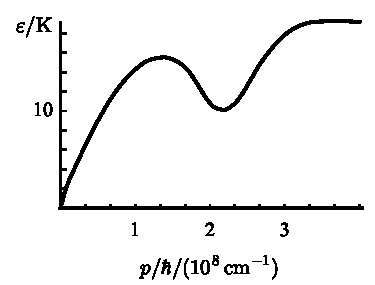
\includegraphics[width=7.2cm]{fig2.pdf}\\[0.3em]
{\small 图 2}
\end{minipage}\par\nopagebreak

\begin{equation*}
F=-NT\ln\frac{eV}{N}\int\mathrm{e}^{-\varepsilon/T}\,\mathrm{d}\tau,\quad
\mathrm{d}\tau=\frac{\mathrm{d}^{3}p}{(2\pi\hbar)^{3}}
\end{equation*}
（见第五卷§41）. 此时应把这个公式中的$N$理解为液体中的旋子数. 但此数本身决定于热力学平衡条件，即决定于自由能取极小值的条件. 令$\partial F/\partial N$等于零，我们求得旋子数为：
\begin{equation}
N_{\text{旋}}=V\int\mathrm{e}^{-\varepsilon/T}\,\mathrm{d}\tau
\label{22.8}
\end{equation}
（当然，它相当于化学势等于零的玻尔兹曼分布）. 相应的自由能值为：
\begin{equation*}
F_{\text{旋}}=-VT\int\mathrm{e}^{-\varepsilon/T}\,\mathrm{d}\tau.
\end{equation*}

现在应将\eqref{22.6}式代入这两个公式. 因为$p_{0}^{2}\gg m^{*}T$，所以对$\mathrm{d}p$积分时，可足够精确地将$p^{2}$换成$p_{0}^{2}$，并将因子$p^{2}$提出积分号外. 被积函数为指数函数时，积分区域可以遍及$-\infty$到$\infty$之间. 最后我们得到：
\begin{equation}
N_{\text{旋}}=\frac{2(m^{*}T)^{1/2}p_{0}^{2}V}{(2\pi)^{3/2}\hbar^{3}}\,\mathrm{e}^{-\varDelta/T},\quad
F_{\text{旋}}=-TN_{\text{旋}}.
\label{22.9}
\end{equation}
因此旋子对熵和热容量的贡献为：
\begin{equation}
S_{\text{旋}}=N_{\text{旋}}\left(\frac{3}{2}+\frac{\varDelta}{T}\right),\quad
C_{\text{旋}}=N_{\text{旋}}\left(\frac{3}{4}+\frac{\varDelta}{T}+\frac{\varDelta^{2}}{T^{2}}\right).
\label{22.10}
\end{equation}

我们看到，各热力学量旋子部分的温度依赖关系基本上是指数函数形式的. 因此，在足够低的温度下（对于液氦，大约低于$0.8\ \mathrm{K}$），旋子部分小于声子部分，而在较高的温度下情况就改变了，这时旋子的贡献超过声子的贡献.

\section{超流性}

具有上述类型能谱的量子液体有一种非凡的性质，称作超流性，即沿毛细管或狭缝流过时不显出任何黏性. 现在我们从研究绝对零度时的液体开始，这时液体处于它的基态，即未被激发的态.

我们来考查以恒定速度$\bm{v}$沿毛细管流动的液体. 由于液体与管壁间的摩擦和液体本身的内摩擦，会发生液体动能的耗散，因而流动将逐渐变慢，这样就显出了黏性的存在.

最好在随液体一起流动的坐标系中来研究液体的流动. 在这个坐标系中氦是静止的，而毛细管壁则以速度$-\bm{v}$运动. 在有黏性存在的情况下，静止的氦也会开始运动起来. 这在物理上是显然的，即液体被管壁粘附时，不可能刚开始就引起液体的整体运动. 运动的出现必然从逐渐激发内部运动开始，也就是从液体中出现元激发开始的.

我们假定在液体中出现一个动量为$\bm{p}$、能量为$\varepsilon(p)$的元激发. 于是，液体的能量$E_{0}$（在液体最初处于静止的坐标系中）就等于这个元激发的能量$\varepsilon$，而液体的动量$\bm{P}_{0}$就等于元激发的动量$\bm{p}$. 现在我们再改用毛细管处于静止的坐标系. 根据力学中熟知的能量和动量的变换公式，对于这个坐标系中液体的能量$E$和动量$\bm{P}$，我们有：
\begin{equation}
E=E_{0}+\bm{P}_{0}\cdot\bm{v}+\frac{Mv^{2}}{2},\quad
\bm{P}=\bm{P}_{0}+M\bm{v},
\label{23.1}
\end{equation}
其中$M$为液体的质量. 将$\varepsilon$，$\bm{p}$代入上式以代换$E_{0},\bm{P}_{0}$，可写成：
\begin{equation}
E=\varepsilon+\bm{p}\cdot\bm{v}+\frac{Mv^{2}}{2}.
\label{23.2}
\end{equation}

$Mv^{2}/2$这一项是流动液体的初动能；表达式$\varepsilon+\bm{p}\cdot\bm{v}$是由于出现激发而引起的能量变化. 因为运动液体的能量应该减少，所以这个能量变化应当是负的：
\begin{equation*}
\varepsilon+\bm{p}\cdot\bm{v}<0.
\end{equation*}
当给定$p$值时，不等式左边的量在$\bm{p}$和$\bm{v}$反平行时具有最小值；因此在任何情况下都应有$\varepsilon-pv<0$，即
\begin{equation}
v>\frac{\varepsilon}{p}.
\label{23.3}
\end{equation}
这个不等式至少对元激发动量$p$的某些值应当是满足的. 所以只要求出量$\varepsilon/p$的极小值，我们便得到沿毛细管运动的液体中可能出现激发的最终条件. 从几何上来说，比值$\varepsilon/p$是从坐标原点（在$p,\varepsilon$平面内）到曲线$\varepsilon=\varepsilon(p)$上某一点所引直线的倾角之正切. 显然，它的极小值决定于从坐标原点向曲线所作的切线之切点. 如果这个极小值不等于零，那么当流速不太大时，液体中不可能出现激发. 这就是说，液体流动不会减慢，即液体显出超流现象.

上面得出的超流性存在的条件，就其实质来说，归结为要求曲线$\varepsilon=\varepsilon(p)$不在坐标原点与横坐标轴相切（撇开可能性很小的情况：即曲线前方的某一点与该轴相切）. 因此，任何能谱，只要其中足够小的激发是声子的话，都会引起超流性.

现在我们来研究温度不等于绝对零度（虽然接近于绝对零度）时的这种液体. 在这种情况下，液体并不处于基态——它含有激发. 这时上述讨论本身自然是有效的，因为在这些讨论中并没有直接利用液体最初处于基态这一情况. 液体相对于管壁的运动，当满足上述条件时仍旧不能在液体中引起新的元激发. 但是，有必要说明在液体中已有的激发是怎样出现的.

为此，我们想象“准粒子气体”作为一个整体以速度$\bm{v}$相对于液体作平动. 作整体运动气体的分布函数可以由静止气体的分布函数求出，这里只要把粒子的能量$\varepsilon$换成$\varepsilon-\bm{p}\cdot\bm{v}$便可，其中$\bm{p}$为粒子的动量. 对于通常的气体来说，这种情况是伽利略相对性原理的直接结果，并且可以简易地借助由一个坐标系变换到另一个坐标系的方法予以证明. 但在我们所研究的这种情况下，不能直接运用这样的论证，因为准粒子气体不是在真空中运动，而是“穿过液体”运动. 虽然如此，从下面的讨论中可以看出，这种论断还是有效的.

设激发气体以速度$\bm{v}$相对于液体运动. 我们来考查这样一个坐标系（坐标系$K$），在这个坐标系中激发气体作为整体处于静止，而液体相应地以速度$-\bm{v}$运动. 根据变换公式\eqref{23.1}，液体在坐标系$K$中的能量$E$与在液体处于静止的坐标系（坐标系$K_{0}$）中的能量$E_{0}$之间的关系式为：
\begin{equation*}
E=E_{0}-\bm{P}_{0}\cdot\bm{v}+\frac{Mv^{2}}{2}.
\end{equation*}
设在液体中出现一个能量为$\varepsilon(p)$（在坐标系$K_{0}$中）的元激发. 这样，在坐标系$K$中液体的附加能量是$\varepsilon-\bm{p}\cdot\bm{v}$，这就证明了上面所作的论断\footnote{对于玻色液体中的准粒子来说，$n(\varepsilon)$ 是分布函数(22.2). 应注意，超流动性条件 $\left(v<\dfrac{\varepsilon}{p}\right)$ 恰好与保证表达式 $n(\varepsilon-\bm{p}\cdot\bm{v})$ 对于任何能量都正定和有限的条件一致.}.

因此准粒子气体（对于单位体积气体）的总动量为：
\begin{equation*}
\bm{P}=\int\bm{p}\,n(\varepsilon-\bm{p}\cdot\bm{v})\,\mathrm{d}\tau.
\end{equation*}
我们假定速度$\bm{v}$很小，于是可以把被积式按$\bm{p}\cdot\bm{v}$的幂展开. 当对矢量$\bm{p}$的方向求积分时零次项消失了，而保留：
\begin{equation*}
\bm{P}=-\int\bm{p}(\bm{p}\cdot\bm{v})\frac{\mathrm{d}n(\varepsilon)}{\mathrm{d}\varepsilon}\,\mathrm{d}\tau,
\end{equation*}
或对$\bm{p}$的方向求平均后，得：
\begin{equation}
\bm{P}=\frac{\bm{v}}{3}\int\left(-\frac{\mathrm{d}n}{\mathrm{d}\varepsilon}\right)p^{2}\,\mathrm{d}\tau.
\label{23.4}
\end{equation}

首先我们看到，准粒子气体的运动伴随着一定质量的迁移：单位体积气体的有效质量决定于\eqref{23.4}式中动量$\bm{P}$与速度$\bm{v}$之间的比例系数. 另一方面，譬如说当液体流经毛细管时，毫不妨碍准粒子同管壁发生碰撞和交换动量. 最终，激发气体将停止不动，就像任何通常的气体流经毛细管时的情况一样.

因此，我们得出下面的基本结论：当温度不等于绝对零度时，一部分质量的液体，其行为如同正常黏性液体一样，在运动时“黏附”在容器壁上；而其余部分质量液体的行为则如同无黏性超流液体. 此时极为重要的是，在“彼此穿过”的这两部分质量的液体之间没有摩擦，即它们之间不发生动量传递. 实际上，在研究作匀速运动的激发气体中的统计平衡时，我们得知：只存在一部分质量液体对于另一部分质量液体的相对运动. 但是，如果在热平衡态中能够发生任何相对运动，那就是说，运动时并不伴有摩擦.

我们强调，把液体当作正常的和超流的两“部分”的“混合体”来研究，只不过是便于描述量子液体中所发生的现象的一种表达方法而已. 这绝不意味着可以把液体真正分成两个部分. 正如用经典术语对量子现象所作的任何描述一样，它并不是完全适合的. 实际上应当说：在量子玻色液体中可以同时存在两种运动，其中每一种运动都与自己的有效质量有关（因此这两种质量之和等于液体总的真实质量）. 这两种运动中，一种是“正常”运动，即具有与通常粘滞液体的运动相同的性质；而另一种是“超流”运动. 这两种运动彼此间不发生动量传递.

因此，就流体动力学的意义来讲，玻色液体的密度可以表示成正常部分与超流部分之和的形式：$\rho=\rho_{n}+\rho_{s}$，其中每一部分都与自己的流体动力学速度$\bm{v}_{n}$和$\bm{v}_{s}$有关. 超流运动的重要性质是它有标势性：
\begin{equation}
\nabla\times\bm{v}_{s}=0.
\label{23.5}
\end{equation}
这一性质是下述事实的宏观表示：波长大的（即动量小的）元激发都是声量子——声子. 因此超流运动的宏观流体动力学，除声振动之外不允许有任何它的振动\footnote{这里所指的是：液体是无界面的. 当存在自由表面时，也可能有表面毛细波出现（这将使表面张力具有一定的温度依赖关系——见习题 1）.}，并由条件\eqref{23.5}来保证（在§26中我们还要讨论它的根据）\footnote{在本教程的另一卷（第六卷）中，对超流液体的流体动力学作了详细的叙述.}.

当$T=0$时，正常部分的密度$\rho_{n}=0$；而液体只能作超流运动. 当温度不等于绝对零度时，$\rho_{n}$由公式\eqref{23.6}给出：
\begin{equation}
\rho_{n}=\frac{1}{3}\int\left(-\frac{\mathrm{d}n}{\mathrm{d}\varepsilon}\right)p^{2}\,\mathrm{d}\tau.
\label{23.6}
\end{equation}

为了计算声子对$\rho_{n}$的贡献，我们在\eqref{23.6}式中取$\varepsilon=up$：
\begin{equation*}
(\rho_{n})_{\text{声}}=-\frac{1}{3u}\int_{0}^{\infty}\frac{\mathrm{d}n}{\mathrm{d}p}\,p^{2}\,\frac{4\pi p^{2}\,\mathrm{d}p}{(2\pi\hbar)^{3}},
\end{equation*}
进行分部积分后，得：
\begin{equation*}
(\rho_{n})_{\text{声}}=\frac{4}{3u}\int_{0}^{\infty}np\,\frac{4\pi p^{2}\,\mathrm{d}p}{(2\pi\hbar)^{3}}
=\frac{4}{3u^{2}}\int\varepsilon n\,\mathrm{d}\tau.
\end{equation*}
这里剩下的积分不是别的，而是单位体积声子气体的能量；取\eqref{22.4}式的能量，最终得：
\begin{equation}
(\rho_{n})_{\text{声}}=\frac{4E_{\text{声}}}{3u^{2}V}=\frac{2\pi^{2}T^{4}}{45\hbar^{3}u^{5}}.
\label{23.7}
\end{equation}

为了计算旋子对$\rho_{n}$的贡献，应注意到：由于旋子可以用玻尔兹曼分布来描述，所以对于旋子来说$\mathrm{d}n/\mathrm{d}\varepsilon=-n/T$，并由\eqref{23.6}式，我们有
\begin{equation*}
(\rho_{n})_{\text{旋}}=\frac{1}{3T}\int p^{2}n\,\mathrm{d}\tau=\frac{\overline{p^{2}}}{3T}\,\frac{N_{\text{旋}}}{V}.
\end{equation*}
我们假定$\overline{p^{2}}=p_{0}^{2}$，这时仍具有足够的精确度，并取\eqref{22.9}式的$N_{\text{旋}}$，我们得到：
\begin{equation}
(\rho_{n})_{\text{旋}}=\frac{p_{0}^{2}N_{\text{旋}}}{3TV}
=\frac{2(m^{*})^{1/2}p_{0}^{4}}{3(2\pi)^{3/2}T^{1/2}\hbar^{3}}\,\mathrm{e}^{-\varDelta/T}.
\label{23.8}
\end{equation}

当温度非常低时，声子对$\rho_{n}$的贡献比旋子的大得多. 在温度$0.6\ \mathrm{K}$时，两者的贡献大约相等，但温度稍高一些，旋子的贡献就占了优势.

随着温度的升高，越来越多质量的液体将变成正常液体. 当达到等式$\rho_{n}=\rho$成立时的温度，超流性将完全消失. 该温度称作液体的$\lambda$点，它是第二级相变点\footnote{温度低于这一点的液氦，称作氦Ⅱ. 诸 $\lambda$ 点在 $P,T$ 平面的相图上构成一条曲线. 这条曲线在 2.19 K 时与液汽平衡曲线相交.}. 定量公式\eqref{23.7}—\eqref{23.8}在$\lambda$点附近当然是不适用的，因为在此处准粒子的浓度变得大了，所以准粒子这一概念本身在很大程度上已失去了意义.

我们还要谈谈溶解在液氦中杂质原子的行为问题；这里假定杂质的浓度如此之低，以致可以认为它的原子间无相互作用［Л.\,Д.\,Ландау, И.\,Я.\,Померанчук, 1948］.

在液体中有杂质原子存在，将引起相应于这种原子在液体中运动的新的能谱支出现；当然，由于杂质原子与液体原子之间的强烈的相互作用，这种运动实际上是液体原子也参与了的集团效应. 这种运动可以用总的守恒动量$\bm{p}$来描述. 因此，在液体中将出现新类型准粒子（其数目等于杂质原子数），这种准粒子能量$\varepsilon_{\text{杂}}(\bm{p})$是动量的某一函数. 在热平衡的情况下，这些准粒子的能量将集中在函数$\varepsilon_{\text{杂}}(\bm{p})$的各极小值中最小的一个附近. 事实上这里所说的杂质是指同位素$^{3}\mathrm{He}$，一些经验资料指明，这个最小值位于$p=0$处；在此位置附近，准粒子能量为
\begin{equation}
\varepsilon_{\text{杂}}(p)=\frac{p^{2}}{2m^{*}_{\text{杂}}},
\label{23.9}
\end{equation}
其中有效质量$m^{*}_{\text{杂}}=2.8\ ^{3}\mathrm{He}$原子质量.

杂质的准粒子同声子和旋子碰撞时发生相互作用，因此杂质准粒子也包含在液体正常部分的成分之中. 由于这些准粒子的浓度很小，它们的热分布为玻尔兹曼分布，并且它们对$\rho_{n}$［按照\eqref{23.6}式的定义］的贡献可由如下公式给出：
\begin{equation}
(\rho_{n})_{\text{杂}}=\frac{N_{\text{杂}}}{V}\,\frac{\overline{p^{2}}}{3T}=\frac{N_{\text{杂}}}{V}\,m^{*}_{\text{杂}},
\label{23.10}
\end{equation}
式中$N_{\text{杂}}/V$是单位体积中杂质原子数.

\begin{xiti}

1. 试求液氦在绝对零度附近时表面张力系数$\alpha$对温度的依赖关系的极限规律（K.\,R.\,Atkins, 1953）.

{\heiti 解：}系数$\alpha$是液体单位表面积的自由能［见第五卷(154.6)式］. 这个量可按照第五卷的公式(64.1)算出来，式中频率$\omega_{0}$现在与表面振动有关. 在二维的情况下，将求和改为（对振动的波矢量）求积分，需要引入因子$\mathrm{d}^{2}k/(2\pi)^{2}$或$2\pi k\,\mathrm{d}k/(2\pi)^{2}$. 进行分部积分后，我们求得：
\begin{equation*}
\alpha=\alpha_{0}+T\int\ln(1-\mathrm{e}^{-\hbar\omega/T})\,\frac{k\,\mathrm{d}k}{2\pi}
=\alpha_{0}-\frac{\hbar}{4\pi}\int\frac{k^{2}\,\mathrm{d}\omega}{\mathrm{e}^{\hbar\omega/T}-1}
\end{equation*}
（$\alpha_{0}$为$T=0$时的表面张力系数）. 在温度足够低的情况下，只有小频率即长波长的振动是主要的. 这种振动形成流体动力学的毛细波，对于这种情况来说，$\omega^{2}=\alpha k^{3}/\rho\approx\alpha_{0}k^{3}/\rho$（$\rho$为液体的密度）. 因此
\begin{equation*}
\alpha=\alpha_{0}-\frac{\hbar}{4\pi}\left(\frac{\rho}{\alpha_{0}}\right)^{2/3}\int_{0}^{\infty}\frac{\omega^{4/3}\,\mathrm{d}\omega}{\mathrm{e}^{\hbar\omega/T}-1}.
\end{equation*}
（式中积分具有迅速的收敛性，因此允许将积分上限换成无穷大）. 算出积分（见第五卷§58脚注）便得到如下结果：
\begin{equation*}
\alpha=\alpha_{0}-\frac{T^{7/3}\rho^{2/3}}{4\pi\hbar^{4/3}\alpha_{0}^{2/3}}\,
\Gamma\!\left(\frac{7}{3}\right)\zeta\!\left(\frac{7}{3}\right)
=\alpha_{0}-0.13\,\frac{T^{7/3}\rho^{2/3}}{\hbar^{4/3}\alpha_{0}^{2/3}}.
\end{equation*}
当温度低到可以把全部液体质量当作是超流质量时，这个结果就是液态$^{4}\mathrm{He}$的了\footnote{在费米液体（液$^{3}$He）中，由于 $T\to 0$ 时粘滞性无限增大，因而我们所研究类型的毛细波（如通常声音的体积波一样）是不存在的.}.

2. 试求运动的超流液体中杂质粒子的色散律$\varepsilon_{\text{杂}}(\bm{p})$，已知在静止液体中该色散律为$\varepsilon^{(0)}_{\text{杂}}(p)$（J.\,Bardeen, G.\,Baym, D.\,Pines, 1967）.

{\heiti 解：}在静止液体中（$T=0$时）加入动量为$\bm{p}_{0}$、质量为$m$的杂质原子后，在液体原来静止的坐标系中液体的能量和动量分别是$E_{0}=\varepsilon^{(0)}_{\text{杂}}(p_{0})$，$\bm{P}_{0}=\bm{p}_{0}$. 而在液体以速度$\bm{v}$运动的坐标系中，根据\eqref{23.1}式则有：
\begin{equation*}
E=\varepsilon^{(0)}_{\text{杂}}(p_{0})+\bm{p}_{0}\cdot\bm{v}+\frac{1}{2}(M+m)v^{2},\quad
\bm{P}=\bm{p}_{0}+(M+m)\bm{v},
\end{equation*}
由此可见，运动液体加入杂质原子时，其能量和动量的改变等于
\begin{equation*}
\bm{\varepsilon}_{\text{杂}}=\bm{\varepsilon}^{(0)}_{\text{杂}}(\bm{p}_{0})+\bm{p}_{0}\cdot\bm{v}+\frac{m\bm{v}^{2}}{2},\quad
\bm{p}=\bm{p}_{0}+m\bm{v}
\end{equation*}
把$\varepsilon_{\text{杂}}$用$p$表达之，我们求得：
\begin{equation*}
\varepsilon_{\text{杂}}(\bm{p})=\varepsilon^{(0)}_{\text{杂}}(\bm{p}-m\bm{v})+\bm{p}\cdot\bm{v}-\frac{m\bm{v}^{2}}{2}.
\end{equation*}
当小$\bm{v}$值时，若精确到一次项，则对于\eqref{23.9}形式的能谱$\varepsilon^{(0)}_{\text{杂}}(p)$，我们有：
\begin{equation*}
\varepsilon_{\text{杂}}(\bm{p})=\frac{p^{2}}{2m^{*}_{\text{杂}}}+\bm{v}\cdot\bm{p}\left(1-\frac{m}{m^{*}_{\text{杂}}}\right).
\end{equation*}

\end{xiti}

\section{液体中的声子}

从声波的经典图像过渡到量子表述时，流体动力学量（液体的密度、速度等等）都要换成用声子的湮没算符$\hat{C}_{\bm{k}}$和产生算符$\hat{C}^{+}_{\bm{k}}$所表达的算符. 现在我们来推导这些物理量的表达公式.

应当注意，在声波的经典描述中，液体密度是要受到微振动的，振动频率和波矢量之间的关系为$\omega=uk$. 液体的速度$\bm{v}$和密度的变化部分$\rho'=\rho-\rho_{0}$（$\rho_{0}$为密度的平衡值）都是同一数量级的小量. 波动中的液体运动是有势的，即它可以用速度标势$\varphi$来描述，并按下式确定速度：
\begin{equation}
\bm{v}=\nabla\varphi,
\label{24.1}
\end{equation}
液体的速度和密度之间是以连续性方程$\partial\rho'/\partial t=-\mathrm{div}(\rho\bm{v})\approx-\rho_{0}\,\mathrm{div}\,\bm{v}$或
\begin{equation}
\frac{\partial\rho'}{\partial t}=-\rho_{0}\Delta\varphi
\label{24.2}
\end{equation}
联系起来的. 声波中的液体能量，可由下列积分得出：
\begin{equation}
E=\int\left(\frac{\rho_{0}\bm{v}^{2}}{2}+\frac{u^{2}\rho'^{2}}{2\rho_{0}}\right)\mathrm{d}^{3}x.
\label{24.3}
\end{equation}
被积式中的第一项是动力学密度，而第二项是液体的内能；这两项分别是小量$\bm{v}$和$\rho'$的平方项.

本来我们可以完全类似于处理晶体中的声子那样（见第五卷§72）进行量子化手续. 但是，这里我们选择了多少不同的方法，它表明方法论上有某些可借鉴之处. 我们首先研究用微观变量（粒子的坐标）表达的液体的密度和速度算符.

在经典理论中，液体的密度$\rho$和质量流密度$\bm{j}$可以表示对所有粒子取和的形式：
\begin{equation*}
\rho(\bm{r})=\sum_{a}m_{a}\delta(\bm{r}_{a}-\bm{r}),\quad
\bm{j}(\bm{r})=\sum_{a}\bm{p}_{a}\,\delta(\bm{r}_{a}-\bm{r})
\end{equation*}
（$\bm{r}_{a}$和$\bm{p}_{a}$为粒子的径矢量和动量）；这两个函数对某一体积的积分，将分别给出该体积中液体的总质量和总动量. 当过渡到量子理论时，这两个函数将换成相应的算符. 密度算符具有同样的形式：
\begin{equation}
\hat{\rho}(\bm{r})=\sum_{a}m_{a}\delta(\bm{r}_{a}-\bm{r}),
\label{24.4}
\end{equation}
而流密度算符为
\begin{equation}
\hat{\bm{j}}(\bm{r})=\frac{1}{2}\sum_{a}\bigl\{\hat{\bm{p}}_{a}\,\delta(\bm{r}_{a}-\bm{r})+\delta(\bm{r}_{a}-\bm{r})\hat{\bm{p}}_{a}\bigr\},
\label{24.5}
\end{equation}
式中$\hat{\bm{p}}_{a}=-\mathrm{i}\hbar\nabla_{a}$是粒子的动量算符\footnote{为简单起见，令系统由一个粒子构成. 可想而知，算符 $\hat{\rho}(\bm{r})=m\delta(\bm{r}_{1}-\bm{r})$ 对波函数 $\psi(\bm{r}_{1})$ 的态求平均，将得出 $\int\psi^{*}(\bm{r}_{1})\hat{\rho}\psi(\bm{r}_{1})\,\mathrm{d}^{3}x_{1}=m\vert\psi(\bm{r})\vert^{2}$. 采用类似的方法，算符 $\hat{\bm{j}}(\bm{r})$ 的平均可给出流密度的正确表达式：$\dfrac{\hbar}{2\mathrm{i}}\{\psi^{*}(\bm{r})\nabla\psi(\bm{r})-\psi(\bm{r})\nabla\psi^{*}(\bm{r})\}$.}.

现在我们来求$\bm{r}$和$\bm{r}'$点算符$\hat{\bm{j}}(\bm{r})$和$\hat{\rho}(\bm{r}')$的对易规则；因为不同粒子的算符是可对易的，所以为简单起见，我们只研究\eqref{24.4}—\eqref{24.5}求和式中的一项. 展开对易子时，将$\delta(\bm{r}_{1}-\bm{r})\nabla_{1}\delta(\bm{r}_{1}-\bm{r}')$形的算符变成如下形状：
\begin{equation*}
\delta(\bm{r}_{1}-\bm{r})\nabla_{1}\delta(\bm{r}_{1}-\bm{r}')
=\delta(\bm{r}_{1}-\bm{r})\bigl(\nabla\delta(\bm{r}-\bm{r}')\bigr)
+\delta(\bm{r}_{1}-\bm{r})\delta(\bm{r}_{1}-\bm{r}')\nabla_{1}.
\end{equation*}
这里第一项中的$\nabla\delta(\bm{r}-\bm{r}')$简单地表示$\delta$函数的梯度；由于这一项里有$\delta(\bm{r}_{1}-\bm{r})$因子，因而可以用$\nabla\delta(\bm{r}-\bm{r}')$代替$\nabla_{1}\delta(\bm{r}_{1}-\bm{r}')$. 最后我们得到：
\begin{equation}
\hat{\bm{j}}(\bm{r})\hat{\rho}(\bm{r}')-\hat{\rho}(\bm{r}')\hat{\bm{j}}(\bm{r})
=-\mathrm{i}\hbar\hat{\rho}\bigl(\nabla\delta(\bm{r}-\bm{r}')\bigr).
\label{24.6}
\end{equation}

现在我们根据定义
\begin{equation*}
\hat{\bm{j}}=\frac{1}{2}\bigl(\hat{\rho}\hat{\bm{v}}+\hat{\bm{v}}\hat{\rho}\bigr)
\end{equation*}
引入液体速度算符$\hat{\bm{v}}$以代替$\hat{\bm{j}}$. 定义算符$\hat{\rho}$和$\hat{\bm{v}}$的对易规则要求：$\hat{\rho}$和$\hat{\bm{j}}$的对易子应得出表达式\eqref{24.6}. 容易验证，为此要取
\begin{equation*}
\hat{\bm{v}}(\bm{r})\hat{\rho}(\bm{r}')-\hat{\rho}(\bm{r}')\hat{\bm{v}}(\bm{r})
=-\mathrm{i}\hbar\bigl(\nabla\delta(\bm{r}-\bm{r}')\bigr).
\end{equation*}
（此时应考虑到算符$\hat{\rho}(\bm{r})$和$\hat{\rho}(\bm{r}')$的明显的可对易）. 最后，取$\hat{\bm{v}}(\bm{r})=\nabla\hat{\varphi}(\bm{r})$，我们便得到密度算符和速度势算符之间的对易规则：
\begin{equation}
\hat{\varphi}(\bm{r})\hat{\rho}'(\bm{r}')-\hat{\rho}'(\bm{r}')\hat{\varphi}(\bm{r})
=-\mathrm{i}\hbar\delta(\bm{r}-\bm{r}')
\label{24.7}
\end{equation}
（这里当然可以写出密度变化部分的算符$\hat{\rho}'=\hat{\rho}-\hat{\rho}_{0}$来代替$\hat{\rho}$）. 规则\eqref{24.7}与粒子坐标和动量之间的对易规则相类似；就此意义来说，$\rho'$和$\varphi$这两个量在该情况下起着正则共轭的广义“坐标”和广义“动量”的作用.

利用建立对易规则\eqref{24.7}的表达式\eqref{24.4}—\eqref{24.5}，我们现在来写出二次量子化表象中的算符$\hat{\varphi}$和$\hat{\rho}'$（即把这两个算符用声子的湮没算符和产生算符表达出来），同时要求它们满足规则\eqref{24.7}. 对此可写成：
\begin{equation*}
\hat{\varphi}(\bm{r})=\frac{1}{\sqrt{V}}\sum_{\bm{k}}
\bigl(A_{\bm{k}}\hat{C}_{\bm{k}}\mathrm{e}^{\mathrm{i}\bm{k}\cdot\bm{r}}
+A^{*}_{\bm{k}}\hat{C}^{+}_{\bm{k}}\mathrm{e}^{-\mathrm{i}\bm{k}\cdot\bm{r}}\bigr),
\end{equation*}
其中$A_{\bm{k}}$为待定系数；求和遍及大而有限的液体体积$V$内的所有波矢量之值\footnote{与粒子 $\psi$ 算符不同，实量算符 $\varphi$ 是厄米的，它同时包含声子的产生算符和湮没算符. 注意，这个性质（与量子电动力学的场算符的性质相同）与声子场中“粒子”数不守恒有关.}. 算符$\hat{C}_{\bm{k}}$，$\hat{C}^{+}_{\bm{k}}$遵从下列玻色对易规则：
\begin{equation}
\hat{C}_{\bm{k}}\hat{C}^{+}_{\bm{k}'}-\hat{C}^{+}_{\bm{k}'}\hat{C}_{\bm{k}}=\delta_{\bm{k}\bm{k}'}.
\label{24.8}
\end{equation}

为了今后引用，我们注意这两个算符不等于零的矩阵元为：
\begin{equation}
\langle n_{\bm{k}}-1\vert\hat{C}_{\bm{k}}\vert n_{\bm{k}}\rangle
=\langle n_{\bm{k}}\vert\hat{C}^{+}_{\bm{k}}\vert n_{\bm{k}}-1\rangle=\sqrt{n_{\bm{k}}}.
\label{24.9}
\end{equation}
式中$n_{\bm{k}}$为声子状态的占有数.

然而，以下我们要用的不是薛定谔算符$\hat{\varphi}(\bm{r})$，而是海森堡算符$\hat{\varphi}(t,\bm{r})$. 只要在下列和式的每一项简单地引入频率为$\omega=uk$的因子$\exp(\pm\mathrm{i}\omega t)$，便容易从$\hat{\varphi}(\bm{r})$得到海森伯算符：
\begin{equation*}
\hat{\varphi}(t,\bm{r})=\frac{1}{\sqrt{V}}\sum_{\bm{k}}
\bigl(A_{\bm{k}}\hat{C}_{\bm{k}}\mathrm{e}^{\mathrm{i}(\bm{k}\cdot\bm{r}-kut)}
+A^{*}_{\bm{k}}\hat{C}^{+}_{\bm{k}}\mathrm{e}^{-\mathrm{i}(\bm{k}\cdot\bm{r}-kut)}\bigr)
\end{equation*}
（对比§9的开头部分中对$\psi$算符所作的叙述）. 密度算符$\hat{\rho}'(t,\bm{r})$应以关系式\eqref{24.2}与算符$\hat{\varphi}(t,\bm{r})$相联系，因此它可由同样的和式得出，但和式中的乘子应以$\mathrm{i}A_{\bm{k}}\rho_{0}k/u$代替$A_{\bm{k}}$. 此后，需要在满足对易规则\eqref{24.7}的条件下确定乘子$A_{\bm{k}}$. 结果得到如下的最终表达式：
\begin{equation}
\begin{gathered}
\hat{\varphi}(t,\bm{r})=\sum_{\bm{k}}\left(\frac{\hbar u}{2V\rho_{0}k}\right)^{1/2}
\bigl(\hat{C}_{\bm{k}}\mathrm{e}^{\mathrm{i}(\bm{k}\cdot\bm{r}-kut)}
+\hat{C}^{+}_{\bm{k}}\mathrm{e}^{-\mathrm{i}(\bm{k}\cdot\bm{r}-kut)}\bigr),\\
\hat{\rho}'(t,\bm{r})=\sum_{\bm{k}}\mathrm{i}\left(\frac{\rho_{0}\hbar k}{2Vu}\right)^{1/2}
\bigl(\hat{C}_{\bm{k}}\mathrm{e}^{\mathrm{i}(\bm{k}\cdot\bm{r}-kut)}
-\hat{C}^{+}_{\bm{k}}\mathrm{e}^{-\mathrm{i}(\bm{k}\cdot\bm{r}-kut)}\bigr).
\end{gathered}
\label{24.10}
\end{equation}

事实上，将这两个表达式代入对易规则\eqref{24.7}的左边，并考虑到\eqref{24.8}式，便得到所要求的$\delta$函数：
\begin{equation*}
\begin{aligned}
&-\mathrm{i}\hbar\,\frac{1}{V}\sum_{\bm{k}}
\bigl(\hat{C}_{\bm{k}}\hat{C}^{+}_{\bm{k}}-\hat{C}^{+}_{\bm{k}}\hat{C}_{\bm{k}}\bigr)
\mathrm{e}^{\mathrm{i}\bm{k}\cdot(\bm{r}-\bm{r}')}={}\\
&\quad=-\frac{\mathrm{i}\hbar}{V}\sum_{\bm{k}}\mathrm{e}^{\mathrm{i}\bm{k}\cdot(\bm{r}-\bm{r}')}
\longrightarrow-\frac{\mathrm{i}\hbar}{V}\int\mathrm{e}^{\mathrm{i}\bm{k}\cdot(\bm{r}-\bm{r}')}\,
\frac{V\,\mathrm{d}^{3}k}{(2\pi)^{3}}
=-\mathrm{i}\hbar\delta(\bm{r}-\bm{r}').
\end{aligned}
\end{equation*}

同样不难证明，在\eqref{24.3}式的积分中以$\hat{\bm{v}}=\nabla\hat{\varphi}$和$\hat{\rho}'$代替$\bm{v}$和$\rho'$，从而得到液体哈密顿量所应具有的形式：
\begin{equation*}
\hat{H}=\sum_{\bm{k}}u\hbar k\left(\hat{C}^{+}_{\bm{k}}\hat{C}_{\bm{k}}+\frac{1}{2}\right),
\end{equation*}
其本征值等于$\sum u\hbar k\,(n_{\bm{k}}+1/2)$. 这正符合能量为$\varepsilon=u\hbar k$的声子的概念.

声波中的液体的能量表达式\eqref{24.3}乃是下列精确表达式的展开式中（在零次项以后）的头两项：
\begin{equation*}
E=\int\left[\frac{\rho\bm{v}^{2}}{2}+\rho e(\rho)\right]\mathrm{d}^{3}x
\end{equation*}
［式中$e(\rho)$是单位质量液体的内能］. 在上述积分中将$\bm{v}$和$\rho$分别换成$\hat{\bm{v}}=\nabla\hat{\varphi}$和$\hat{\rho}=\rho_{0}+\hat{\rho}'$［式中$\hat{\varphi}$和$\hat{\rho}'$由\eqref{24.10}式定义］，则该积分就可作为液体的精确哈密顿量：
\begin{equation}
\hat{H}=\int\left[\frac{\hat{\bm{v}}\cdot\hat{\rho}\hat{\bm{v}}}{2}+\hat{\rho}\,e(\hat{\rho})\right]\mathrm{d}^{3}x
\label{24.11}
\end{equation}
（把动能算符写成对称形式$\hat{\bm{v}}\cdot\hat{\rho}\hat{\bm{v}}\,/\,2$，以便成为厄米算符）. 并且极为重要的是，$\rho$和$\varphi$恰好是正则共轭的“广义坐标和广义动量”，因此必定能通过它们表达出哈密顿量. 这一点可从下述事实看出：\eqref{24.10}的两个算符所遵从的对易规则\eqref{24.7}是一个精确的规则，即在导出它的过程中，任何地方都没利用振动的微小性.

这个哈密顿量的展开式中更高级（三级以上）的各项表达了声振动的非简谐性，用声子图像的术语来说，就是描述了声子的相互作用. 这些项，对于同时改变若干声子占有数的跃迁都有矩阵元. 因而它们起着引起声子各种散射和裂变过程的微扰作用. 此时，算符$\hat{C}_{\bm{k}}$和$\hat{C}^{+}_{\bm{k}}$本身的矩阵元当然具有前面的\eqref{24.9}的形式，正如微扰论中通常的做法一样，这里是利用了使非微扰哈密顿量对角的表象. 我们列出三次项和四次项的表达式：
\begin{equation}
\hat{H}^{(3)}=\int\left[\frac{\hat{\bm{v}}\cdot\hat{\rho}'\hat{\bm{v}}}{2}
+\left(\frac{\mathrm{d}}{\mathrm{d}\rho_{0}}\,\frac{u^{2}}{\rho_{0}}\right)\frac{\hat{\rho}'^{3}}{6}\right]\mathrm{d}^{3}x,
\label{24.12}
\end{equation}
\begin{equation}
\hat{H}^{(4)}=\frac{1}{24}\left(\frac{\mathrm{d}^{2}}{\mathrm{d}\rho_{0}^{2}}\,\frac{u^{2}}{\rho_{0}}\right)\int\hat{\rho}'^{4}\,\mathrm{d}^{3}x.
\label{24.13}
\end{equation}

\section{简并近理想玻色气体}

使用接近于绝对零度时的弱非理想玻色气体模型，可明显地看出玻色型能谱的基本性质. 在这一节里，采取类似于在§6中对费米气体的处理方法来研究这个模型\footnote{下面我们所阐明的方法属于 Н. Н. 博戈留波夫(1947). 他把这种方法运用到玻色气体，是首尾一贯以微观方式推导“量子液体”能谱的最早例证.}. 因而§6所作的关于简并近理想气体模型的普遍性质的全部叙述，同样也适用于现在所研究的情况. 比如说，弱非理想性［气体参数$a(N/V)^{1/3}\ll 1$；$a$为散射长度］的条件，可以照以前的一样，表述为粒子微小动量条件(6.1)的形式：$pa/\hbar\ll 1$\footnote{下面我们将会看到，在简并玻色气体中大多数粒子（“凝聚体”除外）都具有动量 $p\sim\hbar\sqrt{aN/V}$，对于这样的动量，上面指出的不等式确是成立的.}.

玻色子（假设它们是无自旋的）成对相互作用系统的哈密顿量，其形式与(6.6)式的区别只在于无自旋下标：
\begin{equation}
\hat{H}=\sum\frac{p^{2}}{2m}\hat{a}^{+}_{\bm{p}}\hat{a}_{\bm{p}}
+\frac{1}{2}\sum\langle\bm{p}'_{1}\bm{p}'_{2}\vert U\vert\bm{p}_{1}\bm{p}_{2}\rangle
\hat{a}^{+}_{\bm{p}'_{1}}\hat{a}^{+}_{\bm{p}'_{2}}\hat{a}_{\bm{p}_{2}}\hat{a}_{\bm{p}_{1}}
\label{25.1}
\end{equation}
（对全部动量下标求和）. 粒子的湮没算符和产生算符现在满足对易规则：
\begin{equation*}
\hat{a}_{\bm{p}}\hat{a}^{+}_{\bm{p}}-\hat{a}^{+}_{\bm{p}}\hat{a}_{\bm{p}}=1.
\end{equation*}

也和§6中一样，按小动量的假定，将\eqref{25.1}中所有的矩阵元再用它们在零动量时的值来代替，于是
\begin{equation}
\hat{H}=\sum\frac{p^{2}}{2m}\hat{a}^{+}_{\bm{p}}\hat{a}_{\bm{p}}
+\frac{U_{0}}{2V}\sum\hat{a}^{+}_{\bm{p}'_{1}}\hat{a}^{+}_{\bm{p}'_{2}}\hat{a}_{\bm{p}_{2}}\hat{a}_{\bm{p}_{1}}.
\label{25.2}
\end{equation}

把微扰论用于这个哈密顿量，出发点在于下述见解：在理想玻色气体的基态上，全部粒子都处在凝聚体中，即处于能量为零的态上占有数$N_{p=0}\equiv N_{0}=N$；当$\bm{p}\neq 0$时，$N_{p}=0$（见第五卷§62）. 近理想气体在基态和在各弱激发态上，占有数$N_{p}$不等于零，但远小于宏观大数$N_{0}$. $\hat{a}^{+}_{0}\hat{a}_{0}=N_{0}\approx N$远大于1的事实，意味着表达式
\begin{equation*}
\hat{a}_{0}\hat{a}^{+}_{0}-\hat{a}^{+}_{0}\hat{a}_{0}=1
\end{equation*}
小于$\hat{a}_{0}$，$\hat{a}^{+}_{0}$的本身，因此忽略$\hat{a}_{0}$和$\hat{a}^{+}_{0}$的不可对易性时，便可以把它们看作普通的（等于$\sqrt{N_{0}}$的）数.

运用微扰论，意味着现在要在形式上将\eqref{25.2}式的四重求和按小量$\hat{a}_{\bm{p}}$，$\hat{a}^{+}_{\bm{p}}$（$\bm{p}\neq 0$）的幂展开. 展开式的零次项等于
\begin{equation}
\hat{a}^{+}_{0}\hat{a}^{+}_{0}\hat{a}_{0}\hat{a}_{0}=a_{0}^{4}.
\label{25.3}
\end{equation}
一次项是不存在的（由于在这类项里不能遵从动量守恒定律）. 二次项为
\begin{equation}
a_{0}^{2}\sum_{\bm{p}\neq 0}\bigl(\hat{a}_{\bm{p}}\hat{a}_{-\bm{p}}
+\hat{a}^{+}_{\bm{p}}\hat{a}^{+}_{-\bm{p}}+4\hat{a}^{+}_{\bm{p}}\hat{a}_{\bm{p}}\bigr).
\label{25.4}
\end{equation}

限于精确到二次量时，可在\eqref{25.4}式中以总粒子数$N$代换$a_{0}^{2}=N_{0}$. 在\eqref{25.3}这一项里，应估计到更精确的关系式：
\begin{equation*}
a_{0}^{2}+\sum_{\bm{p}\neq 0}\hat{a}^{+}_{\bm{p}}\hat{a}_{\bm{p}}=N.
\end{equation*}
结果，\eqref{25.3}—\eqref{25.4}式各项之和变为
\begin{equation*}
N^{2}+N\sum_{\bm{p}\neq 0}\bigl(\hat{a}_{\bm{p}}\hat{a}_{-\bm{p}}
+\hat{a}^{+}_{\bm{p}}\hat{a}^{+}_{-\bm{p}}+2\hat{a}^{+}_{\bm{p}}\hat{a}_{\bm{p}}\bigr).
\end{equation*}
把它代入\eqref{25.2}式，我们得到哈密顿量的下列表达式：
\begin{equation}
\hat{H}=\frac{N^{2}}{2V}U_{0}
+\sum_{\bm{p}}\frac{p^{2}}{2m}\hat{a}^{+}_{\bm{p}}\hat{a}_{\bm{p}}
+\frac{N}{2V}U_{0}\sum_{\bm{p}\neq 0}\bigl(\hat{a}_{\bm{p}}\hat{a}_{-\bm{p}}
+\hat{a}^{+}_{\bm{p}}\hat{a}^{+}_{-\bm{p}}+2\hat{a}^{+}_{\bm{p}}\hat{a}_{\bm{p}}\bigr).
\label{25.5}
\end{equation}

此表达式的第一项，在一级近似下决定了气体的基态能量$E_{0}$，而它对$N$的微商相应地为$T=0$时的化学势$\mu$：
\begin{equation}
E_{0}=\frac{N^{2}}{2V}U_{0},\quad\mu=\frac{N}{V}U_{0}.
\label{25.6}
\end{equation}
\eqref{25.5}式中其余各项决定了对$E_{0}$的修正和气体弱激发态的能谱.

\eqref{25.5}式中的积分$U_{0}$，还应当通过真实的物理量——散射长度$a$表达出来. 这在二次项中可以直接按照公式(6.2)得出：$U_{0}=4\pi\hbar^{2}a/m$. 而在第一项，则需要用更精确的公式(6.5)表达，该公式顾及了散射幅中的二级玻恩近似. 并且这里所指的是凝聚体两个粒子的碰撞问题，相应地应当在(6.5)式的求和中取$\bm{p}_{1}=\bm{p}_{2}=0$，$\bm{p}'_{1}=-\bm{p}'_{2}\equiv\bm{p}$，因此有：
\begin{equation*}
U_{0}=\frac{4\pi\hbar^{2}a}{m}\left(1+\frac{4\pi\hbar^{2}a}{V}\sum_{\bm{p}\neq 0}\frac{1}{p^{2}}\right),
\end{equation*}
将此式代入\eqref{25.5}式，便得到哈密顿量：
\begin{equation}
\begin{split}
\hat{H}=\frac{2\pi\hbar^{2}a}{m}\,\frac{N^{2}}{V}
\left(1+\frac{4\pi\hbar^{2}a}{V}\sum_{\bm{p}\neq 0}\frac{1}{p^{2}}\right)+{}\\
+\frac{2\pi\hbar^{2}a}{m}\,\frac{N}{V}\sum_{\bm{p}\neq 0}
\bigl(\hat{a}_{\bm{p}}\hat{a}_{-\bm{p}}+\hat{a}^{+}_{\bm{p}}\hat{a}^{+}_{-\bm{p}}
+2\hat{a}^{+}_{\bm{p}}\hat{a}_{\bm{p}}\bigr)
+\sum_{\bm{p}}\frac{p^{2}}{2m}\hat{a}^{+}_{\bm{p}}\hat{a}_{\bm{p}}.
\end{split}
\label{25.7}
\end{equation}

为了确定能级，需要将算符$\hat{a}_{\bm{p}}$，$\hat{a}^{+}_{\bm{p}}$作必要的线性变换，以使哈密顿量变成对角形. 现在我们引入新的算符$\hat{b}_{\bm{p}}$，$\hat{b}^{+}_{\bm{p}}$，根据定义，
\begin{equation*}
\hat{a}_{\bm{p}}=u_{\bm{p}}\hat{b}_{\bm{p}}+v_{\bm{p}}\hat{b}^{+}_{-\bm{p}},\quad
\hat{a}^{+}_{\bm{p}}=u_{\bm{p}}\hat{b}^{+}_{\bm{p}}+v_{\bm{p}}\hat{b}_{-\bm{p}},
\end{equation*}
而且要求它们满足算符$\hat{a}_{\bm{p}}$，$\hat{a}^{+}_{\bm{p}}$所满足的同样的对易关系：
\begin{equation*}
\hat{b}_{\bm{p}}\hat{b}_{\bm{p}'}-\hat{b}_{\bm{p}'}\hat{b}_{\bm{p}}=0,\quad
\hat{b}_{\bm{p}}\hat{b}^{+}_{\bm{p}'}-\hat{b}^{+}_{\bm{p}'}\hat{b}_{\bm{p}}=\delta_{\bm{p}\bm{p}'}.
\end{equation*}
不难看出，为此必定有：$u^{2}_{\bm{p}}-v^{2}_{\bm{p}}=1$. 考虑到这一点，就可把线性变换写成如下形式：
\begin{equation}
\hat{a}_{\bm{p}}=\frac{\hat{b}_{\bm{p}}+L_{\bm{p}}\hat{b}^{+}_{-\bm{p}}}{\sqrt{1-L^{2}_{\bm{p}}}},\quad
\hat{a}^{+}_{\bm{p}}=\frac{\hat{b}^{+}_{\bm{p}}+L_{\bm{p}}\hat{b}_{-\bm{p}}}{\sqrt{1-L^{2}_{\bm{p}}}}.
\label{25.8}
\end{equation}
量$L_{\bm{p}}$应当这样确定，使哈密顿量中消掉非对角项$(\hat{b}_{\bm{p}}\hat{b}_{-\bm{p}},\hat{b}^{+}_{\bm{p}}\hat{b}^{+}_{-\bm{p}})$. 经简单的计算得出：
\begin{equation}
L_{\bm{p}}=\frac{1}{mu^{2}}\left\{\varepsilon(p)-\frac{p^{2}}{2m}-mu^{2}\right\},
\label{25.9}
\end{equation}
其中引入了两个记号：
\begin{equation}
\varepsilon(p)=\left[u^{2}p^{2}+\left(\frac{p^{2}}{2m}\right)^{2}\right]^{1/2},
\label{25.10}
\end{equation}
\begin{equation}
u=\left(\frac{4\pi\hbar^{2}aN}{m^{2}V}\right)^{1/2}.
\label{25.11}
\end{equation}

这时哈密顿量取如下形式：
\begin{equation}
\hat{H}=E_{0}+\sum_{\bm{p}\neq 0}\varepsilon(p)\hat{b}^{+}_{\bm{p}}\hat{b}_{\bm{p}},
\label{25.12}
\end{equation}
式中
\begin{equation}
E_{0}=\frac{N}{2}mu^{2}+\frac{1}{2}\sum_{\bm{p}\neq 0}
\left\{\varepsilon(p)-\frac{p^{2}}{2m}-mu^{2}+\frac{m^{3}u^{4}}{p^{2}}\right\}.
\label{25.13}
\end{equation}

由\eqref{25.12}形式的哈密顿量和算符$\hat{b}_{\bm{p}}$，$\hat{b}^{+}_{\bm{p}}$的玻色对易关系可以推断：$\hat{b}^{+}_{\bm{p}}$和$\hat{b}_{\bm{p}}$乃是遵从玻色统计，能量为$\varepsilon(p)$的准粒子的产生算符和湮没算符. 对角算符$\hat{b}^{+}_{\bm{p}}\hat{b}_{\bm{p}}$的本征值就是动量为$\bm{p}$的准粒子数$n_{\bm{p}}$，而公式\eqref{25.10}决定了准粒子能量对动量的依赖关系（重新用$n_{\bm{p}}$表示准粒子占有数，以区别于气体真实粒子占有数$N_{p}$）. 于是我们所研究气体的弱激发态能谱便完全确定.

量$E_{0}$是气体的基态能量. 以对$V\mathrm{d}^{3}p/(2\pi\hbar)^{3}$求积分代替对离散的$\bm{p}$值（在体积$V$中）求和，经计算得到下列表达式：
\begin{equation}
E_{0}=\frac{2\pi\hbar^{2}aN^{2}}{mV}\left[1+\frac{128}{15}\sqrt{\frac{a^{3}N}{\pi V}}\right]
\label{25.14}
\end{equation}
（李政道，杨振宁，1957）. 关于气体（当$T=0$时）的化学势，相应地有：
\begin{equation}
\mu=\frac{\partial E_{0}}{\partial N}=\frac{4\pi\hbar^{2}aN}{mV}
\left[1+\frac{32}{3}\sqrt{\frac{a^{3}N}{\pi V}}\right].
\label{25.15}
\end{equation}
这两个公式是按$(a^{3}N/V)^{1/2}$的幂展开的前两项. 但是下一项就不能再用上述方法计算了. 这一项应含有体积，如$V^{-2}$，而这一级的量值不仅与二重碰撞，而且也与三重碰撞有关.

当动量值很大（$p\gg mu$）时，\eqref{25.10}式的准粒子能量趋于$p^{2}/2m$，即趋于气体单个粒子的动能.

当动量很小时（$p\ll mu$），则有$\varepsilon\approx up$. 不难看到，系数$u$与气体中的声速相同，因此根据§22的一般证明，这种表式也符合声子的情况. 当$T=0$时，自由能与能量$E_{0}$相等，于是取$E_{0}$的展开式中的主要项，我们求得压强：
\begin{equation*}
P=-\frac{\partial E}{\partial V}=\frac{2\pi\hbar^{2}aN^{2}}{mV^{2}},
\end{equation*}
而得到的声速为$u=\sqrt{\partial P/\partial\rho}$（式中$\rho=mN/V$为气体的密度）并与\eqref{25.11}式相同.

应当指出，在我们所研究的玻色气体模型中，散射长度$a$一定是正值（粒子之间具有排斥相互作用）. 这一点，在形式上由下述事实就可看出，即在已得出的能量公式中，当$a<0$时将会出现虚数项. 条件$a>0$的热力学意义是，在该玻色气体模型中它必须遵从不等式$(\partial P/\partial V)_{T}<0$.

元激发（它们的占有数平均值为$\overline{n}_{\bm{p}}$）的统计分布，当温度不等于零时可简单地由玻色分布公式\eqref{22.2}得出. 气体真实粒子按动量的分布$\overline{N}_{p}$可以用算符$\hat{a}^{+}_{\bm{p}}\hat{a}_{\bm{p}}$求平均的方法算出来. 利用\eqref{25.8}式，并考虑到乘积$\hat{b}_{-\bm{p}}\hat{b}_{\bm{p}}$和$\hat{b}^{+}_{\bm{p}}\hat{b}^{+}_{-\bm{p}}$不具有对角矩阵元这一性质，可得：
\begin{equation}
\overline{N}_{p}=\frac{\overline{n}_{p}+L^{2}_{p}(\overline{n}_{p}+1)}{1-L^{2}_{p}}.
\label{25.16}
\end{equation}
这个表达式，当然只在$\bm{p}\neq 0$时才成立. 动量为零的粒子数为
\begin{equation}
\overline{N}_{0}=N-\sum_{\bm{p}\neq 0}\overline{N}_{p}
=N-\frac{V}{(2\pi\hbar)^{3}}\int\overline{N}_{p}\,\mathrm{d}^{3}p.
\label{25.17}
\end{equation}
特别是，在绝对零度时所有$n_{p}=0$，于是借助\eqref{25.9}式我们可由\eqref{25.16}式得到如下形式的分布函数\footnote{应当指出，具有给定动量值的粒子数极大值（$\sim p^{2}N_{p}$）位于 $p/\hbar\sim\sqrt{aN/V}$ 附近，这里由 $\varepsilon(p)$ 的一个极限表达式过渡到另一个极限表达式. 这种情况已在 90 页的注解中说过了.}：
\begin{equation}
N_{p}=\frac{m^{2}u^{4}}{2\varepsilon(p)\bigl\{\varepsilon(p)+p^{2}/2m+mu^{2}\bigr\}}
\label{25.18}
\end{equation}
（当$T=0$时，$N_{p}$的平均值与精确值相等；因此去掉了字母上的横线）. 当然，玻色气体的非理想性，即使在绝对零度时也会出现动量不为零的粒子；很容易求出\eqref{25.17}式中的积分［其中$N_{p}$由\eqref{25.18}式确定］，因而得出：
\begin{equation}
N_{0}=N\left[1-\frac{8}{3}\sqrt{\frac{Na^{3}}{\pi V}}\right].
\label{25.19}
\end{equation}

最后，我们还要对这里所得的能谱作以下的说明：当$p$小时，微商$\mathrm{d}^{2}\varepsilon/\mathrm{d}p^{2}>0$，就是说$\varepsilon(p)$曲线从初始的切线$\varepsilon=up$起向上弯曲. 在这种情况下（见下面的§34）将发生能谱的不稳定性，这与准粒子（声子）可能具有的自发裂变有关. 但是，由于相应的能级宽度很小（当$p$小时与$p^{5}$成正比），因而并不损及在所研究的近似程度下得到的表达式.

\section{凝聚体的波函数}

在§23里我们已经谈过，在液氦中超流性的出现或消失都是以第二级相变的方式发生的. 这种相变总是与物体性质的某种质变有关. 在液氦处于$\lambda$点的情况，这种质变可以用宏观方法描写为液体超流成分的出现或消失. 以更深刻的微观观点来说，这里所指的乃是液体（真实的!）粒子按动量分布的确定性质. 正是在超流液体中（与非超流液体不同），有限比率的粒子（具有宏观大的粒子数）具有严格等于零的动量；这些粒子在动量空间中构成了玻色-爱因斯坦凝聚体（或简称凝聚体）. 注意，在理想玻色气体中，当$T=0$时气体的全部粒子都变成凝聚体（见第五卷§62）而在近理想气体中，也几乎是所有粒子都变成凝聚体. 在粒子间具有强烈相互作用的玻色液体这种情况，当$T=0$时处于凝聚体中的粒子数的比率绝不能接近于1.

现在我们要说明怎样用$\psi$算符的术语来描述玻色-爱因斯坦凝聚的性质.

对于理想玻色气体——无相互作用的玻色子系统，它的海森伯$\psi$算符可写成如下的显形式\footnote{见(9.3)式. 我们假设气体粒子是无自旋的，因此没有自旋下标. 在(26.1)式中，也考虑了理想玻色气体当 $T=0$ 时化学势 $\mu=0$，因此省略了指数中 $-\mu t/\hbar$ 这一项.}：
\begin{equation}
\hat{\Psi}(t,\bm{r})=\frac{1}{\sqrt{V}}\sum_{\bm{p}}\hat{a}_{\bm{p}}
\exp\left\{\frac{\mathrm{i}}{\hbar}\bm{p}\cdot\bm{r}
-\frac{\mathrm{i}}{\hbar}\,\frac{p^{2}}{2m}\,t\right\}.
\label{26.1}
\end{equation}

在§25中我们已作过说明：可以忽略算符$\hat{a}_{0}$和$\hat{a}^{+}_{0}$的不可对易性，即把这两个算符看作是经典量. 换言之，\eqref{26.1}式的部分$\psi$算符是普通的数，这一部分我们用$\hat{\Xi}$来表达：
\begin{equation}
\hat{\Xi}=\frac{\hat{a}_{0}}{\sqrt{V}}.
\label{26.2}
\end{equation}

为了表达任意玻色液体在一般情况的$\psi$算符的这种性质，应当指出，由于在凝聚体中总具有宏观上大数的粒子，所以当这个粒子数增减1时，实质上并不改变系统的状态，因此可以说，由于向凝聚体添入（或取出）一个粒子，结果由一定的$N$个粒子系统状态得出了$N\pm 1$个粒子系统“同样的”状态\footnote{添入或取出粒子，应想象为进行得无限缓慢. 这样就排除了变化的场对系统的激发.}. 比如说，基态仍然保持为基态. 使凝聚体中粒子数改变1的那部分$\psi$算符用$\hat{\Xi}$，$\hat{\Xi}^{+}$标记，因此按定义就有：
\begin{equation*}
\hat{\Xi}\vert m,N+1\rangle=\Xi\vert m,N\rangle,\quad
\hat{\Xi}^{+}\vert m,N\rangle=\Xi^{*}\vert m,N+1\rangle.
\end{equation*}
这里记号$\vert m,N\rangle$和$\vert m,N+1\rangle$表征系统中仅粒子数不同的两个“相同的”状态，而$\Xi$是某一复数. 这些论断在$N\to\infty$的极限情况下是严格成立的. 因此，$\Xi$这个量的定义应写成如下形式：
\begin{equation}
\begin{gathered}
\lim_{N\to\infty}\langle m,N\vert\hat{\Xi}\vert m,N+1\rangle=\Xi,\\
\lim_{N\to\infty}\langle m,N+1\vert\hat{\Xi}^{+}\vert m,N\rangle=\Xi^{*}.
\end{gathered}
\label{26.3}
\end{equation}
这是液体在给定的有限密度值$N/V$时趋于极限的.

如果把$\psi$算符表成：
\begin{equation}
\hat{\Psi}=\hat{\Xi}+\hat{\Psi}',\qquad
\hat{\Psi}^{+}=\hat{\Xi}^{+}+\hat{\Psi}'^{+}.
\label{26.4}
\end{equation}
则算符的剩余（“非凝聚体”）部分（即$\hat{\Psi}'$，$\hat{\Psi}'^{+}$——译注）将使状态$\vert m,N\rangle$变为与其正交的状态，即矩阵元为\footnote{为了避免误会，我们再不厌其烦地提醒一次：这些等式只对应于“同样”态之间的跃迁！}：
\begin{equation}
\lim_{N\to\infty}\langle m,N\vert\hat{\Psi}'\vert m,N+1\rangle=0,\quad
\lim_{N\to\infty}\langle m,N+1\vert\hat{\Psi}'^{+}\vert m,N\rangle=0.
\label{26.5}
\end{equation}

在$N\to\infty$的极限，状态$\vert m,N\rangle$和$\vert m,N+1\rangle$之间的差别完全消失，就此意义来说，$\Xi$这个量是算符$\hat{\Psi}$对这个态的平均值. 我们强调，此极限值有限是含有凝聚体的这种系统的特点.

等式\eqref{26.3}已透彻表明了$\hat{\Xi}$，$\hat{\Xi}^{+}$的“算符”性质，此外，可以认为它们与$\hat{\Psi}'$，$\hat{\Psi}'^{+}$可对易. 特别是，在对基态求任何平均时，算符$\hat{\Xi}$，$\hat{\Xi}^{+}$将代之以$\Xi$，$\Xi^{*}$（即与经典量的行为相同）. 我们再强调一次：由于凝聚体中粒子数是个宏观量，因而这种近似就意味着只忽略那些相对数量级很小的量$1/N$\footnote{特别是，取这种精确度时，对于系统中粒子数之差相同（不大的）的各不同状态之间的跃迁来说，应当认为算符 $\hat{\Psi}$ 的各跃迁矩阵元都相同.}.

如果波函数的时间依赖关系决定于哈密顿量$\hat{H}'=\hat{H}-\mu\hat{N}$，那么$\Xi$这个量就与时间无关. 事实上，矩阵元$\langle m,N\vert\Xi\vert m,N+1\rangle$正比于
\begin{equation*}
\exp\left\{-\frac{\mathrm{i}t}{\hbar}
\bigl[E(N+1)-E(N)-(N+1)\mu+N\mu\bigr]\right\},
\end{equation*}
但这个指数函数的指数为零，因为精确到$\sim 1/N$时，$E(N+1)-E(N)=\mu$.

在均匀的静止液体中，$\Xi$同样也与坐标无关，因而适当地选取该复变量的相位，容易得出：
\begin{equation}
\Xi=\sqrt{n_{0}},
\label{26.6}
\end{equation}
式中$n_{0}$是单位体积液体中凝聚体的粒子数. 实际上，$\hat{\Xi}^{+}\hat{\Xi}$是凝聚体中的粒子数密度算符，而这个算符的平均值恰好是$n_{0}$.

由于凝聚体的存在，使得玻色液体粒子的密度矩阵本质上有别于通常液体中的密度矩阵. 在均匀玻色液体的任意状态，密度矩阵以下列表达式定义：
\begin{equation}
N\rho(\bm{r}_{1},\bm{r}_{2})
=\langle m,N\vert\hat{\Psi}^{+}(t,\bm{r}_{2})\hat{\Psi}(t,\bm{r}_{1})\vert m,N\rangle,
\label{26.7}
\end{equation}
而且该函数只依赖于$\bm{r}=\bm{r}_{1}-\bm{r}_{2}$这个差［见(7.13)］. 将\eqref{26.4}形式的$\psi$算符代入上式并考虑\eqref{26.3}式和\eqref{26.5}式的性质，我们得到：
\begin{equation}
N\rho(\bm{r}_{1},\bm{r}_{2})=n_{0}+N\rho'(\bm{r}_{1},\bm{r}_{2}).
\label{26.8}
\end{equation}

“非凝聚体”密度矩阵$\rho'$当$\vert\bm{r}_{1}-\bm{r}_{2}\vert\to\infty$时趋近于零；但密度矩阵$\rho$这时趋近于有限的极限值$n_{0}/N$. 这表明在超流液体中存在着通常液体所没有的“远程有序”性，而在通常的液体中当$\vert\bm{r}_{1}-\bm{r}_{2}\vert\to\infty$时总是$\rho\to 0$. 这就是使液体的超流相有别于非超流相的对称性质（В.\,Л.\,金兹堡，Л.\,Д.\,朗道，1950; O.\,Penrose, 1950）.

利用密度矩阵的傅里叶分量，按公式
\begin{equation}
N(\bm{p})=N\int\rho(\bm{r})\,\mathrm{e}^{-\mathrm{i}\bm{p}\cdot\bm{r}}\,\mathrm{d}^{3}x
\label{26.9}
\end{equation}
［比较(7.20)式］可确定出液体粒子按动量的分布. 将\eqref{26.8}式中的$\rho$代入上式，得到：
\begin{equation}
N(\bm{p})=(2\pi)^{3}n_{0}\delta(\bm{p})
+N\int\rho'(\bm{r})\,\mathrm{e}^{-\mathrm{i}\bm{p}\cdot\bm{r}}\,\mathrm{d}^{3}x.
\label{26.10}
\end{equation}
带有$\delta$函数的一项相应于动量严格等于零的粒子的有限概率.

如果在液体中发生超流运动，或液体处于非均匀且不稳定的外界条件下（但该条件只在比原子间距大的距离上才有重大的改变），那就仍旧会发生玻色-爱因斯坦凝聚，但已不能肯定液体将出现$\bm{p}=0$的状态. 以前根据\eqref{26.3}式定义的量$\Xi$，现在是坐标和时间的函数，它具有凝聚态中粒子波函数的意义. 它的归一化条件为$\vert\Xi\vert^{2}=n_{0}$，因此可以把它表达成
\begin{equation}
\Xi(t,\bm{r})=\sqrt{n_{0}(t,\bm{r})}\,\mathrm{e}^{\mathrm{i}\Phi(t,\bm{r})}.
\label{26.11}
\end{equation}
因为有宏观大数的粒子处于凝聚态，这个态的波函数变成为经典的宏观量\footnote{这类似于每个态中光子的占有数很大时，电磁波场强变成了经典量的情况（对照第四卷 §5）.}. 因此，在超流液体中将出现新的宏观态（其中包括热力学平衡态）的特性.

根据波函数\eqref{26.11}算出的流密度是：
\begin{equation*}
\bm{j}_{\text{凝聚}}=\frac{\mathrm{i}\hbar}{2m}
\bigl(\Xi\nabla\Xi^{*}-\Xi^{*}\nabla\Xi\bigr)
=\frac{\hbar}{m}n_{0}\nabla\Phi,
\end{equation*}
式中$m$为液体粒子的质量. 就上式本身意义来说，它是凝聚体粒子宏观的流密度，因而可以把它表为$n_{0}\bm{v}_{0}$的形式，这里$\bm{v}_{0}$是该运动的宏观速度. 对比两个表达式，得：
\begin{equation}
\bm{v}_{0}=\frac{\hbar}{m}\nabla\Phi.
\label{26.12}
\end{equation}

因为这种运动可以在热力学平衡态（用量$\Xi$描述）发生，所以它是一种无耗散的运动，因此\eqref{26.12}式决定了超流运动速度. 这样一来，我们又得出在§23中已经提到的超流运动的性质，即它的标势性. 同时，发现速度势$\varphi$（在精确到常数因子时）与凝聚体波函数的相位是相等的：
\begin{equation}
\varphi=\frac{\hbar}{m}\Phi.
\label{26.13}
\end{equation}

但是为了避免误解，应当强调：虽然凝聚体的速度与液体超流成分的速度相同（即使凝聚体和超流成分在$\lambda$点同时出现），凝聚体密度$mn_{0}$与超流成分密度$\rho_{s}$彼此绝不相同. 毫无疑问，绝没有理由把这两个量混为一谈，混淆这两个量的错误还可以由下列事实看出：在绝对零度时，液体全部质量都是超流的，然而绝非全部液体粒子都处于凝聚体中\footnote{事实上，液氦中凝聚体的密度，看来只是总液体密度的一小部分.}.

\section{凝聚体密度对温度的依赖关系}

凝聚体中粒子数密度在$T=0$时最大，而温度升高时密度降低. 该密度对温度的依赖关系当$T\to 0$时的极限规律，可借助研究宏观量——凝聚体波函数$\Xi$的涨落来求出（R.\,A.\,Ferrell, N.\,Menyhard, H.\,Schmidt, F.\,Schwabl, P.\,Szepfalusy, 1968）.

首先应当提醒，$\Xi$是个经典量，用量子力学形式表达时，它对应于算符$\hat{\Psi}$. 因此，为了计算涨落原则上应该利用这个算符. 另一方面，在绝对零度附近长波振动在宏观量涨落谱中起着主要作用. 液体中这些振动乃是流体动力学宏观方程所描述的声波，因而有可能独立地使$\Xi$量子化来建立对应于这个量的算符.

在这种情况下，对于量$\Xi=\sqrt{n_{0}}\exp(\mathrm{i}\Phi)$来说，直接与公式\eqref{26.13}的超流速度势有关的相位$\Phi$，在长波极限下涨落最强烈. 我们提醒一下，$\varphi$和$\Phi$这两个量都不是单值的，即它们有可加的任意常数. 因此，单值的量$\sqrt{n_{0}}$只能通过$\Phi$的微商表达，所以$\sqrt{n_{0}}$的涨落的傅里叶分量将包含波矢$\bm{k}$的多余的幂，即对于小$\bm{k}$，该分量是很小的.

相位$\Phi$与速度势$\varphi$的关系，可以直接将$\Phi$与描写液体中声子分布的量联系起来. 为此，我们把$\varphi$因而也把$\Phi$看作是二次量子化算符，并根据\eqref{24.10}式通过声子的产生算符和湮没算符将$\hat{\Phi}$展开：
\begin{equation}
\hat{\Phi}=\sum_{\bm{p}}\left(\frac{mu}{2Vnp}\right)^{1/2}
\bigl(\hat{C}_{\bm{p}}\,\mathrm{e}^{\mathrm{i}\bm{p}\cdot\bm{r}/\hbar}
+\hat{C}^{+}_{\bm{p}}\,\mathrm{e}^{-\mathrm{i}\bm{p}\cdot\bm{r}/\hbar}\bigr).
\label{27.1}
\end{equation}
（把非微扰的液体密度写成$\rho=nm$的形式，这里$n$是粒子数密度，并略去下标0）. 如上所述，宏观量$\Xi$的算符，即算符$\hat{\Psi}$的长波部分，可以表成如下形式：
\begin{equation}
\hat{\Psi}=\sqrt{n_{0}}\exp(\mathrm{i}\hat{\Phi}),
\label{27.2}
\end{equation}
式中$n_{0}$为凝聚体的粒子数密度.

首先，我们利用这个公式来计算玻色液体的“非凝聚体”粒子（在小动量值的情况下）按动量的分布. 在单粒子的密度矩阵$\rho(\bm{r}_{1},\bm{r}_{2})$中，当距离$\vert\bm{r}_{1}-\bm{r}_{2}\vert$很大时，就可以利用$\psi$算符的长波表达式\eqref{27.2}：
\begin{equation}
N\rho(\bm{r}_{1},\bm{r}_{2})
=\langle\hat{\Psi}^{+}(\bm{r}_{2})\hat{\Psi}(\bm{r}_{1})\rangle
\approx n_{0}\bigl\langle\mathrm{e}^{-\mathrm{i}\hat{\Phi}^{+}(\bm{r}_{2})}
\mathrm{e}^{\mathrm{i}\hat{\Phi}(\bm{r}_{1})}\bigr\rangle.
\label{27.3}
\end{equation}
这里是对给定温度的液体状态取平均. 由于涨落很小，应当将这个表达式按$\hat{\Phi}$的幂展开，这时只保留前几个未消失的（二次）项. 考虑$\hat{\Phi}^{+}=\hat{\Phi}$，则得：
\begin{equation}
N\rho(\bm{r}_{1},\bm{r}_{2})
=n_{0}-n_{0}\bigl\langle\hat{\Phi}^{2}(r)\bigr\rangle
+n_{0}\bigl\langle\hat{\Phi}(\bm{r}_{2})\hat{\Phi}(\bm{r}_{1})\bigr\rangle.
\label{27.4}
\end{equation}
第三项当$\vert\bm{r}_{2}-\bm{r}_{1}\vert\to\infty$时趋于零，并给出所求的密度矩阵的非凝聚体部分（在均匀液体中第二项根本与$\bm{r}$无关，它给出对凝聚体密度的修正，稍后将用另一种方法计算这个修正）. 利用\eqref{27.1}式，可将非凝聚体部分变成如下形式：
\begin{equation*}
\begin{aligned}
N\rho'(\bm{r}_{1},\bm{r}_{2})
&=\frac{n_{0}mu}{2Vn}\sum_{\bm{p}}\frac{1}{p}
\bigl\{\langle\hat{C}^{+}_{\bm{p}}\hat{C}_{\bm{p}}\rangle
\mathrm{e}^{-\mathrm{i}\bm{p}\cdot(\bm{r}_{1}-\bm{r}_{2})/\hbar}
+\langle\hat{C}_{\bm{p}}\hat{C}^{+}_{\bm{p}}\rangle\cdot
\mathrm{e}^{\mathrm{i}\bm{p}\cdot(\bm{r}_{1}-\bm{r}_{2})/\hbar}\bigr\}=\\
&=\frac{n_{0}mu}{Vn}\sum_{\bm{p}}\frac{1}{p}
\left(n_{\bm{p}}+\frac{1}{2}\right)
\mathrm{e}^{\mathrm{i}\bm{p}\cdot(\bm{r}_{1}-\bm{r}_{2})/\hbar},
\end{aligned}
\end{equation*}
式中
\begin{equation*}
n_{\bm{p}}=\bigl[\mathrm{e}^{pu/T}-1\bigr]^{-1}.
\end{equation*}
将求和变为求积分，有：
\begin{equation}
N\rho'(\bm{r}_{1},\bm{r}_{2})=\frac{n_{0}mu}{n}\int
\frac{n_{p}+1/2}{p}\,
\mathrm{e}^{\mathrm{i}\bm{p}\cdot(\bm{r}_{1}-\bm{r}_{2})/\hbar}\,
\frac{\mathrm{d}^{3}p}{(2\pi\hbar)^{3}}
\label{27.5}
\end{equation}
当然，此表达式只对来自小动量$\bm{p}$（即$\hbar/p$大于原子间距离）的贡献成立. \eqref{27.5}式中的被积式可直接确定粒子按动量的分布：
\begin{equation}
N(\bm{p})=\frac{n_{0}mu}{np}\left(n_{p}+\frac{1}{2}\right).
\label{27.6}
\end{equation}
当$T=0$时，此公式给出：
\begin{equation}
N(\bm{p})=\frac{n_{0}mu}{2np}
\label{27.7}
\end{equation}
（J.\,Gavoret, Ph.\,Nozi\'eres, 1964），当$T\neq 0$时，$up\ll T$；于是
\begin{equation}
N(\bm{p})=\frac{n_{0}mT}{np^{2}}.
\label{27.8}
\end{equation}
（P.\,C.\,Hohenberg, P.\,C.\,Martin, 1965）现在可以确定凝聚体密度对温度的依赖关系. 按定义，我们有：
\begin{equation}
n_{0}(T)=n-\int N(\bm{p})\,\frac{\mathrm{d}^{3}p}{(2\pi\hbar)^{3}}.
\label{27.9}
\end{equation}

如果直接将\eqref{27.6}式代入此公式，则积分由于零振动而发散. 这种情形，与\eqref{27.6}式不适用于大动量$p$有关，并意味着不能只用这种方法计算凝聚体在$T=0$时的密度值，该密度值在这里应认为是给定的量. 为了确定所求的对温度的依赖关系，需要从$n_{0}(T)$中减去它在$T=0$时的值，这时积分已收敛. 结果我们得到：
\begin{equation}
\begin{aligned}
\frac{n_{0}(T)-n_{0}(0)}{n_{0}(0)}
&=-\frac{mu}{n}\int\frac{n_{p}}{p}\,\frac{\mathrm{d}^{3}p}{(2\pi\hbar)^{3}}={}\\
&=-\frac{mT^{2}}{2\pi^{2}nu\hbar^{3}}\int_{0}^{\infty}\frac{x\,\mathrm{d}x}{\mathrm{e}^{x}-1}
=-\frac{mT^{2}}{12nu\hbar^{3}}.
\end{aligned}
\label{27.10}
\end{equation}

在计算时，我们忽略了液体总密度对温度的依赖关系；由于液体的热膨胀（与声子的激发有关）正比于更高的温度的幂次——$T^{4}$（见第五卷§67），所以作这样忽略是合理的\footnote{已得出的对于任何玻色液体都成立的各公式，当然与 §25 中得出的弱非理想玻色气体的各公式是一致的. 在比较时，应考虑对于弱非理想气体来说 $n_{0}\approx n$，而 $p$ 小的条件为：$p\ll mu\sim\hbar(an)^{1/2}$.}.

\section{超流密度在$\lambda$点附近的行为}

在§23中已经谈过，玻色液体的超流密度的比率$\rho_{s}/\rho$随着温度的升高而减小，并在第二级相变点（称作液体的$\lambda$点）变为零. $\lambda$点的温度$T_{\lambda}$是压强$P$的函数；方程$T=T_{\lambda}(P)$决定了$P,T$平面相图上诸$\lambda$点所构成的曲线.

在第二级相变的普遍理论中，物体状态的改变是以表征物体对称性质的序参数的行为来描述的. 对于玻色液体的$\lambda$相变来说，凝聚体波函数$\Xi$就起着这种参数的作用，在§26中曾说过，它描述液体中的“远程有序”性. $\Xi$是一个复数就说明：序参数有两个分量，并且系统的有效哈密顿量（见第五卷§147）只与$\vert\Xi\vert^{2}$有关，也就是说，对于$\Xi\to\mathrm{e}^{\mathrm{i}\alpha}\Xi$（$\alpha$为任意实数）的变换，哈密顿量是不变的.

看来有关液氦中$\lambda$相变的实验资料证明：对这种相变，朗道相变理论得以适用的区域并不存在. 因为不论在$\lambda$点邻域的任何地方（即不论在$\vert T-T_{\lambda}\vert\ll T_{\lambda}$范围内的任何地方）都不满足第五卷(146.15)这一判据. 因此，描述这种相变的性质需要运用第二级相变的涨落理论，该理论可以将各种量对温度的依赖关系相互联系起来.

序参数（因而也包括凝聚体的密度$n_{0}$）当$T\to T_{\lambda}$时对温度的依赖关系由临界指数$\beta$给出（见第五卷§148）：
\begin{equation}
\vert\Xi\vert=\sqrt{n_{0}}\propto(T_{\lambda}-T)^{\beta}.
\label{28.1}
\end{equation}

但我们更感兴趣的是超流密度$\rho_{s}$的行为问题. 为计算$\rho_{s}$，我们来研究这样的液体：在该液体中凝聚体波函数的相位$\Phi$在空间作缓慢的变化. 这就是说，在液体中发生速度为\eqref{26.12}式的宏观超流运动，单位体积液体相应的动能为：
\begin{equation}
\frac{\rho_{s}v_{s}^{2}}{2}=\rho_{s}\,\frac{\hbar^{2}}{2m^{2}}\bigl(\nabla\Phi\bigr)^{2}.
\label{28.2}
\end{equation}

此表达式也可以用于序参数的长波涨落. 根据标度不变性的假设，在相变点邻域决定涨落状况的唯一的长度参数，乃是涨落的关联半径$r_{c}$. 因而，该参数也用来确定这样数量级的距离，在该距离内相位$\Phi$的涨落变化的数量级为1；所以，涨落速度平方的平均值随温度的变化规律为：
\begin{equation*}
\overline{v_{s}^{2}}\propto r_{c}^{-2}\propto(T_{\lambda}-T)^{2\nu}.
\end{equation*}
式中$\nu$为关联半径的临界指数. 另一方面，因为热力学量在相变点的特性恰好与长波涨落有关，自然可以认为：在该点的邻域，涨落动能\eqref{28.2}与液体热力学势的奇异部分一样按同样规律即$(T_{\lambda}-T)^{2-\alpha}$（这里$\alpha$是热容量$C_{p}$的临界指数）随温度改变. 因此求得：
\begin{equation*}
\rho_{s}\overline{v_{s}^{2}}\propto\rho_{s}(T_{\lambda}-T)^{2\nu}\propto(T_{\lambda}-T)^{2-\alpha}.
\end{equation*}
从而$\rho_{s}\propto(T_{\lambda}-T)^{2-\alpha-2\nu}$. 最后，考虑关系式
\begin{equation}
3\nu=2-\alpha
\label{28.3}
\end{equation}
（根据标度不变性的假设得出——见第五卷§149），最终得到：
\begin{equation}
\rho_{s}\propto(T_{\lambda}-T)^{(2-\alpha)/3}.
\label{28.4}
\end{equation}

此式将$\lambda$点附近的$\rho_{s}$和热容量分别对温度的依赖关系相互联系起来（B.\,D.\,Josephson, 1966）.

我们注意到从第五卷(148.13)和(148.17)可得出关系式：
\begin{equation}
\alpha+2\beta+\nu(2-\zeta)=2.
\label{28.5}
\end{equation}
其中$2\beta$为决定$n_{0}$对温度依赖关系的指数. 此\eqref{28.5}式可以表成
\begin{equation*}
2\beta=(2-\alpha)(1-\zeta)/3.
\end{equation*}
的形式. 对于液氦，指数$\alpha$和$\zeta$事实上是很小的. 因此，相当精确地有$2\beta\approx(2-\alpha)/3\approx 2/3$，于是
\begin{equation*}
\rho_{s}\sim n_{0}\sim(T_{\lambda}-T)^{2/3}.
\end{equation*}

鉴于\eqref{28.4}式的重要性，最好做另一更形式化的推导. 为此计算相位$\Phi$涨落的关联函数.

由于只对经典涨落感兴趣，我们首先求出与其相关的自由能的变化，因对能量和对自由能的微小附加值是相等的. 此变化可以根据\eqref{28.2}式直接写为
\begin{equation}
\Delta F=\rho_{s}\,\frac{\hbar^{2}}{2m^{2}}\int(\nabla\Phi)^{2}\,\mathrm{d}V
\label{28.6}
\end{equation}

遵循第五卷§116在计算密度涨落关联函数时所用的方法，将$\Delta\Phi$按坐标展成傅里叶级数：
\begin{equation}
\Delta\Phi=\sum_{\bm{k}}\Phi_{\bm{k}}\,\mathrm{e}^{\mathrm{i}\bm{k}\cdot\bm{r}},\qquad
\Phi_{-\bm{k}}=(\Phi_{\bm{k}})^{*}.
\label{28.7}
\end{equation}
将此式代入\eqref{28.6}. 按$\mathrm{d}V$积分的结果，对于$\bm{k}\neq-\bm{k}'$的多项均为零. 剩下的积分归于乘以$V$，因此得到
\begin{equation*}
\Delta F=\rho_{s}\,\frac{\hbar^{2}}{2m^{2}}\,V\sum_{\bm{k}}k^{2}\vert\Phi_{\bm{k}}\vert^{2}.
\end{equation*}

根据热力学涨落的普遍理论，这表明
\begin{equation}
(\vert\Phi_{\bm{k}}\vert^{2})=\frac{T}{V}\,\frac{m^{2}}{\rho_{s}\hbar^{2}}\,\frac{1}{k^{2}},\quad
\langle\Phi_{\bm{k}}\Phi_{\bm{k}'}\rangle=0,\quad\bm{k}\neq\bm{k}'
\label{28.8}
\end{equation}

现在可以将\eqref{28.7}式代入关联函数表达式$\varphi(\vert\bm{r}_{1}-\bm{r}_{2}\vert)=\langle\Delta\Phi(\bm{r}_{1})\Delta\Phi(\bm{r}_{2})\rangle$，并用\eqref{28.8}式进行平均. 经简单计算得出
\begin{equation}
\varphi(r)=\frac{T}{V}\,\frac{m^{2}}{\rho_{s}\hbar^{2}}\sum_{\bm{k}}\frac{1}{k^{2}}\,
\mathrm{e}^{\mathrm{i}\bm{k}\cdot\bm{r}}
=T\,\frac{m^{2}}{\rho_{s}\hbar^{2}}\int\frac{1}{k^{2}}\,
\mathrm{e}^{\mathrm{i}\bm{k}\cdot\bm{r}}\,\frac{\mathrm{d}^{3}k}{(2\pi)^{3}}.
\label{28.9}
\end{equation}
利用单位电荷库仑势的傅里叶分量$\dfrac{4\pi}{k^{2}}$，即可写出积分答案：
\begin{equation}
\varphi(r)=T\,\frac{m^{2}}{4\pi\rho_{s}\hbar^{2}}\,\frac{1}{r}.
\label{28.10}
\end{equation}

公式\eqref{28.10}适于$\lambda$点以下的一切温度（在足够大的距离上）. 在邻近$T_{\lambda}$，此公式适于$r\ll r_{c}$的距离上在此区域可以忽略序参数模的较小的涨落并认为此参数的涨落等于$\Delta\Xi=\mathrm{i}\sqrt{n_{0}}\,\Delta\varphi$. 于是，相位$\varphi(r)$的关联函数乘以$n_{0}$便与序参数的关联函数$\rho(r)=\langle\Delta\Xi^{*}(r_{2})\Delta\Xi(r_{1})\rangle$一致了. （应指出，考虑$\Xi$的波函数意义，$\rho$就是液体的密度矩阵.）在适用区域的边界，当$r\sim r_{c}$序参数关联函数在数量级上应该跟普遍表达式(148.7)（参阅第五卷）相一致：
\begin{equation}
\rho(r)\sim r^{-(1+\zeta)}.
\label{28.11}
\end{equation}
当$r\sim r_{c}$，函数$\rho(r)$等于$n_{0}\varphi(r)$，便得出
\begin{equation*}
\rho_{s}\sim n_{0}r_{c}^{-\zeta}\sim(T_{\lambda}-T)^{2\beta-\nu\zeta}.
\end{equation*}
利用\eqref{28.3}和\eqref{28.5}容易信服此温度依赖关系同\eqref{28.4}式一致.
